\subsection {Session 8, Exercise 6}
\label{8f6}

\lineparagraph {Exercise}

Prove that the following Karp-reductions exist:

\begin{enumerate}[a)]
    \item $SUBSETSUM \prec HAM$
    \item $CONNECTED \prec 3-SAT$
    \item $CONNECTED \prec BIPARTITE$
\end{enumerate}

where $CONNECTED$ is the language of connected graphs, while $BIPARTITE$ is the language of bipartite graphs.

\lineparagraph {Solution}

Quick rundown here of what is what:

\begin{itemize}
    \item $SUBSETSUM$ is $NP$-complete, we learned this
    \item $HAM$ is $NP$-complete, we learned this.
    \item $CONNECTED$ is in $P$, because we run a $BFS$ on a graph from any vertex to see if it's connected, if it reaches all vertices, then it is. $BFS$ is a polynomial time algorithm.
    \item $3-SAT$ is $NP$-complete, we learned this.
    \item $BIPARTITE$, we have shown in \nameref{8f1} that it is also in $P$.
\end{itemize}

\textbf{a)}

\begin{itemize}
    \item Is an $NP$-complete problem Karp-reducible to another $NP$-complete problem? Yes.
    \item $NP$-complete means it is both in $NP$ and $NP$-hard.
    \item Let's use the $NP$ fact for the left side, the $NP$-hard fact for the right side.
    \item Is a language that is in $NP$ Karp-reducible to another that is $NP$-hard? Yes. This is the definition of $NP$-hardness, all languages in $NP$ can be Karp-reduced onto it.
\end{itemize}

\textbf{b)}

\begin{itemize}
    \item Is a language in $P$ Karp-reducible to a language that is $NP$-complete?
    \item $P$ is a subset of $NP$, so the question is exactly the same as in $a)$: left side is in $NP$, right side is $NP$-hard, so the Karp-reduction must exist. (See \nameref{8f1}, second solution for a different approach, for when you actually have to give the Karp-reduction.)
\end{itemize}

\textbf{c)}
\begin{itemize}
    \item Is a language in $P$ Karp-reducible to another language in $P$?
    \item Yes, a language in $P$ is basically Karp-reducible to anything, for similar reasons as in \nameref{8f1}, second solution:
    \item The Karp-reduction transformation function allows us to run any polynomial algorithm. Since the language on the left side is in $P$, we can start by solving it in polynomial time.
    \item Then When we know the solution, we are faced with one more difficulty: we have to go through the solver algorithm for the language on the right side. We can't directly output the $YES$ or $NO$ answer.
    \item So we will come up with a specific input that we know will make the solver say $YES$ and another that will make the solver say $NO$.
    \item To make the $BIPARTITE$ solver say yes, we input this graph:
\end{itemize}

\begin{center}
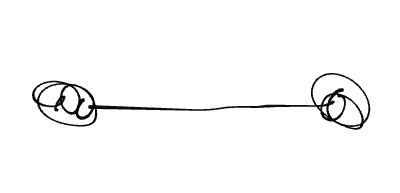
\includegraphics[width=100px]{./08/06/bipartite_yes.png}
\end{center}

\begin{itemize}
    \item To make the $BIPARTITE$ solver say no, we input this graph:
\end{itemize}

\begin{center}
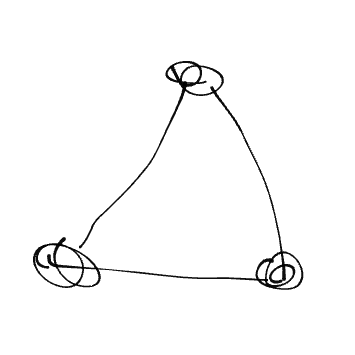
\includegraphics[width=100px]{./08/06/bipartite_no.png}
\end{center}